\section{\hspace{1em} Числени симулации}
\begin{frame}[t]{Стойности на параметри}
  \begin{table}
    \begin{small}
      \begin{tabular}{ |c ||c c c c c c|  }
        % \hhline{~------}
        \hline
        \multirow{2}{*}{Параметър}& \multicolumn{2}{c}{Набор 1}& \multicolumn{2}{c}{Набор 2} & \multicolumn{2}{c|}{Набор 3}\\
        & М. 1 & М. 2 & М. 1 & М. 2 & М. 1 & М. 2\\
        \hline
        % \hhline{~------}
        $\beta_{vh}$ & \multicolumn{2}{c}{$0.5$} & \multicolumn{2}{c}{$0.5$}  & \multicolumn{2}{c|}{$0.5$}\\
        $\beta_{hv}$ & \multicolumn{2}{c}{$0.1$} & \multicolumn{2}{c}{$0.1$} & \multicolumn{2}{c|}{$0.1$}\\
        $a_i$ & $0.12$ & $0.18$ & $0.158$ & $0.159$ & $0.15$ & $0.24$\\
        $M_i$ & $6 \times 10^7$ & $1.6 \times 10^8$ & $7320950$ & $4695340$ & $7320950$ & $4695340$\\
        $\mu_i$ & $\frac{1}{21}$ & $\frac{1}{15}$ & $0.032$ & $0.046$ & $0.0397$ & $0.0335$\\
        $\tau$ & \multicolumn{2}{c}{$10$} & \multicolumn{2}{c}{$10$} & \multicolumn{2}{c|}{$10$}\\
        $N_i$ & $8 \times 10^6$ & $2 \times 10^7$ & $9377980$ & $4467650$ & $755440$ & $3945290$\\
        $\gamma_i$ & \multicolumn{2}{c}{$\frac{1}{14}$} & $0.0627$ & $0.0576$ & $0.0735$ & $0.0622$\\
        $p_{ij}$ & \multicolumn{6}{c|}{различни ($p_{i1}+p_{i2}=1$)}\\
        $\kappa$ & \multicolumn{2}{c}{$0.44$} & \multicolumn{2}{c}{$0.37$} & \multicolumn{2}{c|}{$0.38$}\\
        $\bar{u}_i$ & $0.15$ & $0.3$ & $0.39$ & $0.12$ & $0.35$ & $0.3$\\
        $\bar{I}_i$ & $0.1$ & $0.14$ & $0.065$ & $0.12$ & $0.09$ & $0.09$\\
        \hline
      \end{tabular}
    \end{small}
    \caption{Таблица със стойностите на параметрите от таблица \ref{tbl:Definitions} за числени симулации}
    \label{tbl:ParameterValues}
  \end{table}
\end{frame}

\begin{frame}[t]{Числени симулации на равновесните точки}
  \begin{figure}[h]
    \centering
    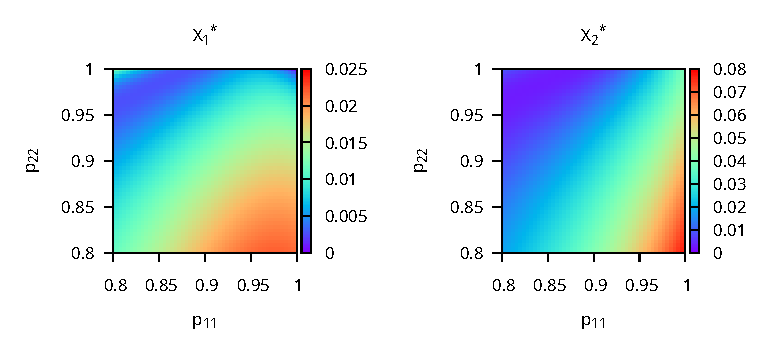
\includegraphics[width=\textwidth]{equilibrium-poster.pdf}
    \caption{Равновесните точки на \eqref{eq:TheDimensionlessProblem}} с параметрите от набор 1 от таблица \ref{tbl:ParameterValues}
    \label{fig:EquilibriumPoints-poster}
  \end{figure}
\end{frame}

\begin{frame}[t]{Числени симулации на равновесните точки}
  \begin{figure}[h]
    \centering
    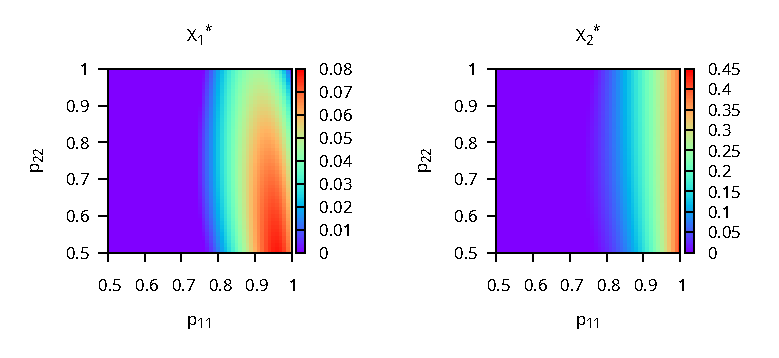
\includegraphics[width=\textwidth]{equilibrium-03-19-16-12-04.pdf}
    \caption{Равновесните точки на \eqref{eq:TheDimensionlessProblem}} с параметрите от набор 2 от таблица \ref{tbl:ParameterValues}
    \label{fig:EquilibriumPoints-03-19-16-12-04}
  \end{figure}
\end{frame}

\begin{frame}[t]{Числени симулации на равновесните точки}
  \begin{figure}[h]
    \centering
    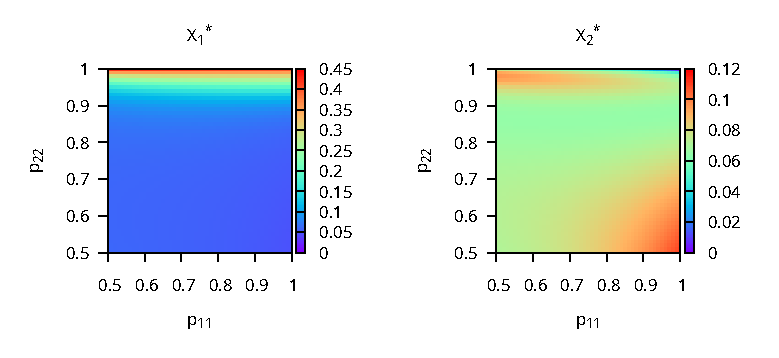
\includegraphics[width=\textwidth]{equilibrium-03-19-16-58-19.pdf}
    \caption{Равновесните точки на \eqref{eq:TheDimensionlessProblem}} с параметрите от набор 3 от таблица \ref{tbl:ParameterValues}
    \label{fig:EquilibriumPoints-03-19-16-58-19}
  \end{figure}
\end{frame}

\begin{frame}[t]{Числени симулации на решението}
  \begin{figure}[h]
    \centering
    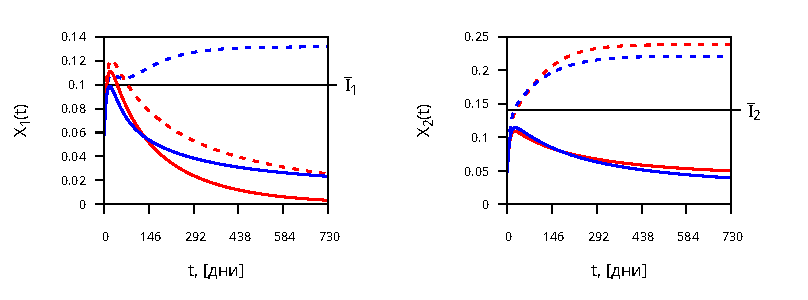
\includegraphics[width=\textwidth]{solution-poster.pdf}
    \caption{Решението на \eqref{eq:TheDimensionlessProblem} с параметрите от набор 1 таблица \ref{tbl:ParameterValues} и $\mathbf{z}_0=(0.0572, 0.048, 0.052, 0.044)^T$.\\
      Пунктирано: без употреба на репелент ($\mathbf{u}(t) \equiv \mathbf{0}$), плътно: максимална употреба на репелент ($\mathbf{u}(t) \equiv \bar{\mathbf{u}}$).\\
    Червено: без мобилност ($p_{11}=p_{22}=1$), синьо: с мобилност ($p_{11}=p_{22}=0.85$)}
    \label{fig:Solution-poster}
  \end{figure}
\end{frame}

\begin{frame}[t]{Числени симулации на решението}
  \begin{figure}[h]
    \centering
    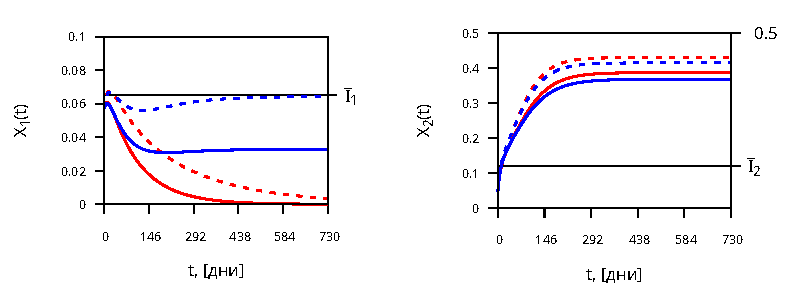
\includegraphics[width=\textwidth]{solution-03-19-16-12-04.pdf}
    \caption{Решението на \eqref{eq:TheDimensionlessProblem} с параметрите от набор 2 от таблица \ref{tbl:ParameterValues} и $\mathbf{z}_0=(0.0572, 0.048, 0.052, 0.044)^T$.\\
      Пунктирано: без употреба на репелент ($\mathbf{u}(t) \equiv \mathbf{0}$), плътно: максимална употреба на репелент ($\mathbf{u}(t) \equiv \bar{\mathbf{u}}$).\\
    Червено: без мобилност ($p_{11}=p_{22}=1$), синьо: с мобилност ($p_{11}=0.99, p_{22}=0.9$).}
    \label{fig:Solution-03-19-16-12-04}
  \end{figure}
\end{frame}

\begin{frame}[t]{Числени симулации на решението}
  \begin{figure}[h]
    \centering
    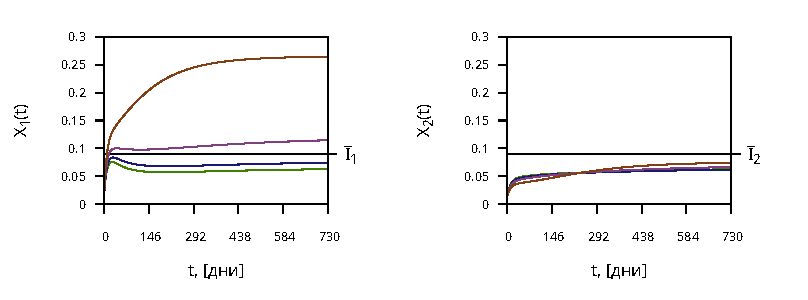
\includegraphics[width=\textwidth]{solution-03-19-16-58-19.pdf}
    \caption{Решението на \eqref{eq:TheDimensionlessProblem} с параметрите от набор 3 от таблица \ref{tbl:ParameterValues} и $\mathbf{z}_0=(0.02, 0.015, 0.04, 0.03)^T$, максимална употреба на репелент ($\mathbf{u}(t) \equiv \bar{\mathbf{u}}$).
      За четирите криви е фиксирано $p_{11}=0.93$, а $p_{22}$ е различно.\\
    Зелено: много висока мобилност ($p_{22}=0.85$), синьо: висока мобилност ($p_{22}=0.88$), лилаво: средна мобилност ($p_{22}=0.92$), кафяво: ниска мобилност ($p_{22}=0.97$).}
    \label{fig:Solution-03-19-16-58-19}
  \end{figure}
\end{frame}

\begin{frame}[t]{Числено приближение на $V(\bar{\boldsymbol{I}}, \bar{\boldsymbol{u}})$ }
  \begin{table}[H]
    \centering
    \begin{tabular}{ | c| c c c c|}
      \hline
      \backslashbox{$p_{22}$}{$p_{11}$}& 0.8 & 0.85 & 0.9 & 0.95 \\
      \hline
      0.95 & 3.427 & 3.447 & 3.467 & 3.486\\
      0.9 & 3.468 & 3.487 & 3.507 & 3.527\\
      0.85 & 3.498 & 3.517 & 3.536 & 3.554\\
      0.8 & 3.519 & 3.540 & 3.559 & 3.580\\
      \hline
    \end{tabular}
    \caption{4-мерната мярка на ядрото на слаба инвариантност на Белман $V(\bar{\boldsymbol{I}}, \bar{\boldsymbol{u}})$ за различни стойности на мобилността с параметрите от набор 1 от таблица \ref{tbl:ParameterValues}. Стойността при случая без мобилност е взета за референтна.}
    \label{tbl:ViabilityKernel-poster}
  \end{table}
\end{frame}
